%% ----------------------------------------------------------------
%% Thesis.tex -- MAIN FILE (the one that you compile with LaTeX)
%% ---------------------------------------------------------------- 

% Set up the document
\documentclass[a4paper, 11pt, oneside]{Thesis}  % Use the "Thesis" style, based on the ECS Thesis style by Steve Gunn
\graphicspath{{Figures/}}  % Location of the graphics files (set up for graphics to be in PDF format)
%Table
%\usepackage{deluxetable}
\usepackage{capt-of}
% Include any extra LaTeX packages required
\usepackage[square, numbers, comma, sort&compress]{natbib}  % Use the "Natbib" style for the references in the Bibliography
\usepackage{verbatim}  % Needed for the "comment" environment to make LaTeX comments
\usepackage{vector}  % Allows "\bvec{}" and "\buvec{}" for "blackboard" style bold vectors in maths
\hypersetup{urlcolor=blue, colorlinks=true}  % Colours hyperlinks in blue, but this can be distracting if there are many links.
\usepackage[utf8]{inputenc}
%\usepackage{arabtex}
\usepackage{capt-of}
\usepackage{epstopdf} % Automatically convert EPS figures to PDF
%\usepackage{english}
%\usepackage[arabic]{babel}
\usepackage[arabic, english]{babel}
%\usepackage{csquotes}
\usepackage[T1, T2A]{fontenc}
%\usepackage[LFE,LAE]{fontenc}
%\textLR{Latin text}
%\usepackage[LAE]{fontenc}
%\usepackage[english]{babel}
%\usepackage{hyperref}
%\hypersetup{draft}
%\selectlanguage{australian}
%\usepackage[english,bidi=default]{babel}
%\babelprovide[import,main]{arabic}
%\babelfont[arabic]{rm}{Amiri}
\usepackage{amsmath} % for the equation* environment

%Import the natbib package and sets a bibliography  and citation styles
\usepackage{natbib}
\bibliographystyle{abbrvnat}
\setcitestyle{authoryear,open={(},close={)}} %Citation-related commands


%% ----------------------------------------------------------------
\begin{document}

%\foreignlanguage{english}
%\selectlanguage{english}

\frontmatter %Begin Roman style (i, ii, iii, iv...) page numbering




    % Set up the Title Page
\title  { {Nuclear Network Calculations of Hydrogen Burning in Nova Thermodynamic Trajectories} \\ \vspace{2mm} %5mm vertical space
 {\selectlanguage{arabic} حسابات الشبكة النووية لاحتراق الهيدروجين في المسارات الديناميكية الحرارية للمستعرات العظمى }}
\authors  {\texorpdfstring
            {\href{https://orcid.org/my-orcid?orcid=0009-0005-1195-7013}{Alshaima Jasim Abdalla ALNAQBI} }\\ 
            }
\authorsa  {\texorpdfstring
            {\href{https://orcid.org/my-orcid?orcid=0009-0005-1195-7013}{\selectlanguage{arabic} \textRL{{الشيماء جاسم عبدالله النقبي} }}}
           {.....}
            }
\addresses  {\groupname\\\deptname\\\univname}  % Do not change this here, instead these must be set in the "Thesis.cls" file, please look through it instead
\date       {\today}
\subject    {}
\keywords   {}
\maketitle
%\footrule{\textcopyright UoS - 2022}
%{\selectlanguage{arabic} \babelfont[arabic]{rm}{Amiri} \maketitle }
%% ----------------------------------------------------------------

\setstretch{1.3}  % It is better to have smaller font and larger line spacing than the other way round

% Define the page headers using the FancyHdr package and set up for one-sided printing
\fancyhead{}  % Clears all page headers and footers
%\fancyfoot{} % Clears all page headers and footers
%\rhead{\thepage}  % Sets the right side header to show the page number
%\cfoot{\thepage}  % Sets the center right side header to show the page number
%\lhead{}  % Clears the left side page header
%\rhead{}  % Clears the left side page header

%\pagestyle{fancy}  % Finally, use the "fancy" page style to implement the FancyHdr headers
%\pagestyle{empty}  % No headers or footers for the following pages

\renewcommand{\headrulewidth}{0pt}
  \thispagestyle{fancy}
  %\thispagestyle{fancy}
  \cfoot{\thepage}  % Sets the center right side header to show the page number
  
%\addtotoc{Committee Decision}  % Add the "Abstract" page entry to the Contents

%\committe{
%\addtocontents{toc}{\vspace{1em}}  % Add a gap in the Contents, for aesthetics
%	%%% 0dApproval/ %%%

%\thispagestyle{empty}

\vspace*{+1em}
\begin{center}
\textbf{\Large Committee Decision}
%\vspace*{+2em}
%Dissertation in partial fulfillment of the requirements for the degree of\\
%
%MASTER OF Physics\\
%\vspace*{+1em}
%Al al-Bayt University\\
%Department of Physics\\
%\vspace*{+1em}

\end{center}

\vspace*{+1em}

This thesis \textbf{ "Title of the thesis" }was successfully defended and approved on dd month 2022.

\vspace*{+1em}

\begin{tabular}{ l l  }
\textbf{\Large  Examination Committee} &               \textbf{\Large Signature}  \\
  &      \\
  Prof. Mashhoor A. Al-Wardat, (Supervisor)&              ..........................................\\
  Department of Applied Physics and Astronomy\\ College of Sciences, University of Sharjah\\ 27272 Sharjah, UAE\\
\color{blue}{\href{mailto:malwardat@sharjah.ac.ae}{malwardat@sharjah.ac.ae}} \\

  & \\
    Prof. xxxxxxxxxxxxxxxxxxx, (Co-Supervisor)&              ..........................................\\
  Department of Applied Physics and Astronomy\\  University of Sharjah, 27272 Sharjah, UAE\\
\color{blue}{\href{mailto:malwardat@sharjah.ac.ae}{malwardat@sharjah.ac.ae}} \\

  & \\
     Dr. xxxxxxxxxxxxxxxxxxxxx (Internal Examiner)&              ..........................................\\
  Department of Applied Physics and Astronomy\\  University of Sharjah, 27272 Sharjah, UAE\\
\color{blue}{\href{mailto:malwardat@sharjah.ac.ae}{malwardat@sharjah.ac.ae}} \\

 & \\
     Dr. xxxxxxxxxxxxxxxxxxxxx (External Examiner)&              ..........................................\\
  Department of Applied Physics and Astronomy\\  University of Sharjah, 27272 Sharjah, UAE\\
\color{blue}{\href{mailto:malwardat@sharjah.ac.ae}{malwardat@sharjah.ac.ae}} \\

\end{tabular}

%\vspace*{+4em}

%\begin{center}
%[16/5/2021]
%\end{center}

%}

\clearpage  % Declaration ended, now start a new page
%% ----------------------------------------------------------------
% Declaration Page required for the Thesis, your institution may give you a different text to place here
%\cfoot{\thepage}  % Sets the center right side header to show the page number

%\pagestyle{empty}  % Finally, use the "fancy" page style to implement the FancyHdr
%\renewcommand{\headrulewidth}{0pt}
 % \thispagestyle{fancy}
  %\thispagestyle{fancy}
  %\cfoot{\thepage}  % Sets the center right side header to show the page number
%\Declaration{
%\addtocontents{toc}{\vspace{1em}}  % Add a gap in the Contents, for aesthetics

%I, AUTHOR NAME, declare that this thesis titled, `THESIS TITLE' and the work presented in it are my own. I confirm that:

%\begin{itemize} 
%\item[\tiny{$\blacksquare$}] This work was done wholly or mainly while in %candidature for a research degree at this University.
 
%\item[\tiny{$\blacksquare$}] Where any part of this thesis has previously been submitted for a degree or any other qualification at this University or any other institution, this has been clearly stated.
 
%\item[\tiny{$\blacksquare$}] Where I have consulted the published work of others, this is always clearly attributed.
 
%\item[\tiny{$\blacksquare$}] Where I have quoted from the work of others, the source is always given. With the exception of such quotations, this thesis is entirely my own work.
 
%\item[\tiny{$\blacksquare$}] I have acknowledged all main sources of help.
 
%\item[\tiny{$\blacksquare$}] Where the thesis is based on work done by myself jointly with others, I have made clear exactly what was done by others and what I have contributed myself.
%\\
%\end{itemize}
 
 
%%%Signed:\\
%%\rule[1em]{25em}{0.5pt}  % This prints a line for the signature
 
%Date:\\
%\rule[1em]{25em}{0.5pt}  % This prints a line to write the date
%}
%\clearpage  % Declaration ended, now start a new page

%% ----------------------------------------------------------------
% The "Funny Quote Page"
%\pagestyle{empty}  % No headers or footers for the following pages

%\null\vfill
% Now comes the "Funny Quote", written in italics
%\textit{``Once you stop learning, you start dying ''}

%\begin{flushright}
%Albert Einstein
%\end{flushright}

%\vfill\vfill\vfill\vfill\vfill\vfill\null
%\clearpage  % Funny Quote page ended, start a new page
%% ----------------------------------------------------------------

% The Abstract Page
\addtotoc{Abstract}  % Add the "Abstract" page entry to the Contents
\abstract{ 
\addtocontents{toc}{\vspace{1em}}  % Add a gap in the Contents, for aesthetics

Classical novae are explosive events in which hydrogen-rich material accreted onto a white dwarf undergoes thermonuclear burning under rapidly changing temperature and density conditions. This project will investigate nova hydrogen burning using dynamic single-zone nuclear reaction network calculations performed with NucNet Tools, with initial abundances adopted from the Lodders solar abundance data.

Preliminary calculations have been completed for two thermodynamic prescriptions: an idealised exponential expansion model and a nova trajectory-based model. These results show that the adopted thermodynamic history strongly affects the final CNO isotopic composition. The exponential model produces early burning followed by freeze-out, while the trajectory model develops a delayed temperature peak that leads to stronger hot-CNO processing.

The proposed work will extend these preliminary results by using larger nuclear networks and by analysing reaction flows, nuclear timescales, and quasi-equilibrium behaviour. The study aims to identify the physical conditions and key nuclear reactions that control CNO isotope production and freeze-out in nova-like environments.

}

\clearpage  % Abstract ended, start a new page


\addtotoc{\textRL{\selectlanguage{arabic}{الملخص}}}  % Add the "Abstract" page entry to the Contents

\abstracta {
\addtocontents{toc}{\vspace{1em}}  % Add a gap in the Contents, for aesthetics
{\selectlanguage{arabic}
%\addtocontents{toc}{\vspace{1em}}  % Add a gap in the Contents, for aesthetics.
تُعدّ المستعرات التقليدية أحداثاً انفجارية يحدث فيها احتراق نووي حراري للمادة الغنية بالهيدروجين المتراكمة على سطح قزم أبيض، وذلك تحت ظروف متغيرة بسرعة من درجة الحرارة والكثافة. يهدف هذا المشروع إلى دراسة احتراق الهيدروجين في بيئات المستعرات التقليدية باستخدام حسابات شبكة تفاعلات نووية ديناميكية موضعية، وذلك بالاعتماد على حزمة \textLR{NucNet Tools}، مع استخدام الوفرة الابتدائية المأخوذة من \textLR{Bergemann (2025)} للوفرة الشمسية.

أُنجزت حسابات أولية باستخدام وصفين مختلفين للتطور الحراري: نموذج تمدد أسي مثالي، ونموذج يعتمد على مسار حراري خاص بالمستعرات التقليدية. تُظهر هذه النتائج أن التاريخ الحراري المعتمد يؤثر بقوة في التركيب النظائري النهائي لعناصر دورة الكربون والنيتروجين والأكسجين. ففي النموذج الأسي يحدث الاحتراق في المراحل المبكرة ثم يتبعه تجمد في الوفرة النووية، بينما يُظهر نموذج المسار الحراري قمة حرارية متأخرة تؤدي إلى معالجة نووية أقوى ضمن دورة CNO الساخنة.

سيعمل هذا المشروع على توسيع هذه النتائج الأولية من خلال استخدام شبكات نووية أكبر، وتحليل تدفقات التفاعلات، والمقاييس الزمنية النووية، والسلوك شبه المتزن. وتهدف الدراسة إلى تحديد الظروف الفيزيائية والتفاعلات النووية الأساسية التي تتحكم في إنتاج نظائر دورة \textLR{CNO} وحدوث الثبات في معدلات تخلق الانوية في البيئات الشبيهة بالمستعرات التقليدية.
}
}

\clearpage  % Abstract ended, start a new page
%% ----------------------------------------------------------------
% Begin the Dedication page

\mainmatter	  % Begin normal, numeric (1,2,3...) page numbering

\setstretch{1.3}  % Return the line spacing back to 1.3

%\pagestyle{empty}  % Page style needs to be empty for this page
%\dedicatory{To the one who bears a lot from me\ldots \ldots to my family and friends\ldots}

%\addtocontents{toc}{\vspace{2em}}  % Add a gap in the Contents, for aesthetics

\clearpage

\setstretch{1.3}  % Reset the line-spacing to 1.3 for body text (if it has changed)

% The Acknowledgements page, for thanking everyone
%\acknowledgements{
%\addtocontents{toc}{\vspace{1em}}  % Add a gap in the Contents, for aesthetics

%The acknowledgements and the people to thank go here, don't forget to include your project advisor\ldots

%}
%\clearpage  % End of the Acknowledgements
%% ----------------------------------------------------------------

\pagestyle{fancy}  %The page style headers have been "empty" all this time, now use the "fancy" headers as defined before to bring them back


%% ----------------------------------------------------------------
\lhead{\emph{Contents}}  % Set the left side page header to "Contents"
\tableofcontents  % Write out the Table of Contents

%% ----------------------------------------------------------------
\lhead{\emph{List of Figures}}  % Set the left side page header to "List if Figures"
\listoffigures  % Write out the List of Figures

%% ----------------------------------------------------------------
\lhead{\emph{List of Tables}}  % Set the left side page header to "List of Tables"
\listoftables  % Write out the List of Tables

%% ----------------------------------------------------------------
\setstretch{1.5}  % Set the line spacing to 1.5, this makes the following tables easier to read
\clearpage  % Start a new page
%\lhead{\emph{Abbreviations}}  % Set the left side page header to "Abbreviations"
%\listofsymbols{ll}  % Include a list of Abbreviations (a table of two columns)
%{
% \textbf{Acronym} & \textbf{W}hat (it) \textbf{S}tands \textbf{F}or \\
%\textbf{CME} & \textbf{C}oronal \textbf{M}ass \textbf{E}jection \\

%\textbf{MF} & \textbf{M}agnetic \textbf{F}ield \\
%}

%% ----------------------------------------------------------------
%\clearpage  % Start a new page
%\lhead{\emph{Physical Constants}}  % Set the left side page header to "Physical Constants"
%\listofconstants{lrcl}  % Include a list of Physical Constants (a four column table)
%{
%Constant Name & Symbol & = & Constant Value (with units) \\
%Speed of Light & $c$ & $= $ & $ 2.997\ 924\ 58\ \times 10^{8}\ \mbox{ms}^{-\mbox{1}}$ \\

%Earth Radius & $R_\oplus $&$ = $&$ 6,371\mbox{km} $\\
%}

%% ----------------------------------------------------------------
\clearpage  %Start a new page
%\lhead{\emph{Symbols}}  % Set the left side page header to "Symbols"
%\listofnomenclature{lll}  % Include a list of Symbols (a three column table)
%{
% symbol & name & unit \\
%$B$ & tesla &  $\frac{kg}{As^2 } \ $ \\
%$p$ & power &  Js$^{-1}$ \\
%& & \\ % Gap to separate the Roman symbols from the Greek

%}
%% ----------------------------------------------------------------
% End of the pre-able, contents and lists of things


%% ----------------------------------------------------------------
%\mainmatter	  % Begin normal, numeric (1,2,3...) page numbering
\rhead{\textbar \thepage}  % Sets the right side header to show the page number
\pagestyle{fancy}  % Return the page headers back to the "fancy" style
\renewcommand{\headrulewidth}{0.5pt}
\fancyfoot{} % Clears all page headers and footers


%\cfoot{\footnote{\hline}}  % Sets the center right side header to show the page number 

%\text M.Sc. Thesis • Name of the student • Dep. of Applied Physics and Astronomy • UoS • 2021
%\rhead{\thepage}  % Sets the right side header to show the page number
%\cfoot{\thepage}  % Sets the center right side header to show the page number
%\lhead{}  % Clears the left side page header
%\rhead{}  % Clears the left side page header

% Include the chapters of the thesis, as separate files
% Just uncomment the lines as you write the chapters
%M.Sc. Thesis • Name of the student • Dep. of Applied Physics and Astronomy • UoS • 2021
%\addtotoc{Chapter 1}
% Chapter 1

\chapter{Introduction} % Write in your own chapter title
\label{Chapter1}
\lhead{\emph{Introduction}} % Write in your own chapter title to set the page header
\fancyfoot[CE,CO]{\hline \\ \small Alshaima Alnaqbi  • Dep. of Applied Physics and Astronomy • UoS • 2026}


\section{Overview}

Classical nova are explosive stellar events produced in close binary systems when hydrogen-rich material is accreted onto the surface of a white dwarf. As the accreted envelope becomes compressed and heated, thermonuclear burning is triggered under degenerate or partially degenerate conditions, leading to a rapid increase in temperature and energy generation. During this phase, hydrogen burning proceeds mainly through the CNO cycles, and the resulting nucleosynthesis can significantly modify the abundances of light and intermediate-mass nuclei. Isotopes such as $^{14}N, ^{15}N, ^{14}O$, and $^{15}O$ are important tracers of the hot-CNO reaction flow and the freeze-out conditions after the temperature declines.

Single-zone nuclear reaction network calculations provide a useful first step for studying nova nucleosynthesis. Although they do not capture the full hydrodynamic structure of a nova envelope, they allow the nuclear physics and thermodynamic effects to be examined in a controlled way. In such calculations, the abundance evolution is followed under a prescribed temperature and density history. The adopted thermodynamic evolution is therefore a key ingredient: an idealised exponential expansion can describe rapid cooling in a simple analytic form, while a thermodynamic trajectory profile can represent a more realistic nova-like heating and cooling history.

In this work, we perform dynamic single-zone nuclear network calculations of hydrogen burning under nova-like conditions using two thermodynamic prescriptions: an exponential expansion model and a trajectory-based model. We focus on the evolution of the diagnostic abundance ratio $(15N+15O)/(14N+14O)$, which is sensitive to the competition between proton captures, beta decays, and freeze-out in the hot-CNO cycle. We first compare the abundance evolution

\subsection{Previous Studies }


Hydrogen burning in classical novae proceeds primarily through the CNO cycles, where oxygen isotopes play a central role in both energy generation and nucleosynthesis. Early foundational studies in nuclear astrophysics established the importance of the CNO cycle in stellar environments, particularly under high-temperature conditions relevant to explosive hydrogen burning \cite{RolfsRodney1988,Adelberger2011}. These works showed that isotopes such as $^{16}\mathrm{O}$, $^{17}\mathrm{O}$, and $^{18}\mathrm{O}$ participate in reaction chains that regulate the overall reaction flow and final isotopic abundances.

Detailed nova simulations have demonstrated that oxygen isotopes are highly sensitive to the underlying white dwarf composition and peak thermodynamic conditions. In particular, \cite{JoseHernanz1998} showed that nucleosynthesis differs significantly between CO and ONe white dwarfs, leading to distinct abundance patterns for oxygen and nearby elements. This highlights the importance of initial composition and thermodynamic evolution in determining oxygen isotope production.

Single-zone nuclear network calculations have been widely used to study hydrogen burning under prescribed thermodynamic trajectories. Reaction rate libraries developed by \cite{Iliadis2002} enable detailed post-processing studies, while \cite{Iliadis2001} specifically investigated the sensitivity of isotopic abundances from oxygen to calcium to variations in thermonuclear reaction rates. These studies demonstrated that uncertainties in key proton-capture reactions can significantly affect the predicted abundances of oxygen isotopes.

The impact of nuclear reaction rate uncertainties has been further explored using statistical approaches. Monte Carlo studies by \cite{Parikh2013,Parikh2014} identified the most critical reactions influencing nova nucleosynthesis, including those involving oxygen isotopes. In particular, reactions such as $^{17}\mathrm{O}(p,\alpha)$ and $^{18}\mathrm{F}(p,\alpha)$ play a crucial role in determining the final abundance distribution within the CNO region.

Thermodynamic trajectories also have a strong influence on hydrogen burning pathways. The work of \cite{Downen2013} demonstrated that variations in temperature and density histories can lead to significant differences in nucleosynthesis outcomes. Similarly, \cite{Denissenkov2014} emphasized the role of mixing processes and accretion history in shaping the thermodynamic evolution, which in turn affects oxygen isotope production during nova outbursts.

Advances in nuclear physics input have improved the reliability of nova models. Updated thermonuclear reaction rate evaluations by \cite{Iliadis2010} and uncertainty analyses by \cite{Champagne2014} provide essential constraints for modeling hydrogen burning processes. These improvements are particularly important for reactions involving oxygen isotopes, where experimental data are still limited.

Recent reviews have summarized progress in the field and highlighted remaining challenges. For example, \cite{Jose2020} emphasized the interplay between nuclear reaction rates, thermodynamic conditions, and mixing processes in shaping nova nucleosynthesis. Their work confirms that oxygen isotopes serve as key tracers of the physical conditions governing explosive hydrogen burning.

Overall, previous studies demonstrate that single-zone nuclear network calculations are powerful tools for investigating hydrogen burning in nova environments. They provide important insights into how thermodynamic trajectories and nuclear reaction rates influence the synthesis and destruction of oxygen isotopes within the CNO cycles.


\section{Problem of the Study}

Classical novae are important astrophysical sites for explosive hydrogen burning and the production of light and intermediate-mass isotopes. During a nova outburst, accreted hydrogen-rich material on the surface of a white dwarf undergoes thermonuclear burning under rapidly changing temperature and density conditions. The resulting nucleosynthesis is strongly influenced by the hot-CNO cycle, in which isotopes such as $^{14}\mathrm{N}$, $^{15}\mathrm{N}$, $^{14}\mathrm{O}$, and $^{15}\mathrm{O}$ play a central role.

A major difficulty in modelling nova nucleosynthesis is understanding how the assumed thermodynamic history affects the final abundance pattern. Idealized single-zone calculations often use simple analytic prescriptions, such as exponential expansion and cooling, while more realistic calculations may use thermodynamic trajectory profiles extracted from nova models. These different approaches can lead to different nuclear processing histories and different final isotopic ratios. Therefore, it is necessary to investigate how sensitive the nucleosynthetic outcome is to the adopted temperature-density evolution.

Preliminary calculations show that the diagnostic abundance ratio
\[
R_{15/14} =
\frac{^{15}\mathrm{N}+^{15}\mathrm{O}}
{^{14}\mathrm{N}+^{14}\mathrm{O}}
\]
is strongly affected by the thermodynamic prescription. In the exponential model, rapid cooling leads to early nuclear burning followed by freeze-out, while in the trajectory-based model, a delayed temperature peak produces stronger hot-CNO processing and a larger final enhancement of this ratio. However, further analysis is required to determine whether these results remain robust when larger nuclear networks are used, and to identify the reaction flows, nuclear timescales, and quasi-equilibrium behavior that control the final abundances.

The problem addressed in this study is therefore the need to determine how thermodynamic history and network size influence CNO isotope production during nova hydrogen burning. The study will focus on dynamic single-zone nuclear reaction network calculations and will examine the physical mechanisms responsible for the production and freeze-out of $^{15}\mathrm{N}$-rich material.

\subsection{Goals of the Study}

The main goal of this study is to investigate hydrogen burning in nova-like environments using dynamic single-zone nuclear reaction network calculations. The study aims to compare idealized exponential thermodynamic evolution with trajectory-based thermodynamic evolution and to determine how these different prescriptions affect the final CNO isotopic composition.

The specific goals of the study are:

\begin{enumerate}
    \item To reproduce and analyse preliminary single-zone nova hydrogen-burning calculations using exponential and thermodynamic trajectory models.

    \item To study the time evolution of key CNO isotopes, especially $^{14}\mathrm{N}$, $^{15}\mathrm{N}$, $^{14}\mathrm{O}$, and $^{15}\mathrm{O}$.

    \item To quantify the evolution of the diagnostic abundance ratio
    \[
    R_{15/14} =
    \frac{^{15}\mathrm{N}+^{15}\mathrm{O}}
    {^{14}\mathrm{N}+^{14}\mathrm{O}},
    \]
    and compare its final value for different thermodynamic histories.

    \item To extend the calculations to larger nuclear networks and examine whether the final CNO isotopic outcome depends on network size.

    \item To identify the dominant reaction flows in the hot-CNO cycle and determine the main nuclear bottlenecks controlling the abundance evolution.

    \item To compute nuclear and thermodynamic timescales in order to determine when active burning occurs and when the abundance pattern freezes out.

    \item To investigate whether parts of the CNO cycle approach quasi-equilibrium or steady-flow behaviour during the active burning phase.

    \item To provide a physical interpretation of how temperature-density evolution controls the production of $^{15}\mathrm{N}$-rich material in nova hydrogen burning.
\end{enumerate} % Introduction
%\addtotoc{Chapter 2}
% Chapter 2

\chapter{Methodology} % Write in your own chapter title
\label{Chapter2}
\lhead{\emph{Methodology}} % Write in your own chapter title to set the page header
\fancyfoot[CE,CO]{\hline \\ \small Alshaima Alnaqbi  • Dep. of Applied Physics and Astronomy • UoS • 2026}

This chapter describes the computational methodology that will be used to study nova hydrogen burning through dynamic single-zone nuclear reaction network calculations. The calculations will be performed using prescribed thermodynamic histories and different nuclear network sizes in order to investigate how temperature-density evolution and network completeness affect the final nucleosynthetic outcome. The main focus will be on the production and evolution of CNO isotopes, especially $^{14}\mathrm{N}$, $^{15}\mathrm{N}$, $^{14}\mathrm{O}$, and $^{15}\mathrm{O}$.

The nuclear reaction network calculations in this study will be performed using the NucNet Tools package developed by Bradley S. Meyer and collaborators at Clemson University. NucNet Tools provides a computational framework for constructing nuclear reaction networks, preparing zone input files, evolving nuclear abundances under prescribed thermodynamic conditions, and analysing the resulting nucleosynthesis output. In this work, the package will be used to carry out dynamic single-zone hydrogen-burning calculations for both exponential and trajectory-based thermodynamic histories. The initial nuclear abundances will be adopted from the \cite{bergemann2025chemical} solar abundance data, which provide the starting composition for the nova-like burning calculations. These initial abundances will be used to construct the input zone files.

\section{Single-Zone Nuclear Reaction Network}

The study will be based on single-zone nuclear reaction network calculations. In this approximation, the burning material is represented by one homogeneous zone. The temperature and density of the zone are prescribed as functions of time, while the nuclear abundances are evolved by solving a coupled system of ordinary differential equations. Although this approach does not describe the full hydrodynamic structure of a nova envelope, it is useful for isolating the effects of nuclear reactions, thermodynamic history, and freeze-out on the final abundance pattern.

The abundance of each nuclide will be expressed in terms of the molar abundance,

\begin{equation}
    Y_i = \frac{X_i}{A_i}
\end{equation}

where $X_i$ is the mass fraction of nuclide $i$ and $A_i$ is its mass number. The time evolution of the abundance vector will be calculated using a nuclear reaction network that includes the relevant charged-particle reactions, beta decays, and other nuclear processes important for hydrogen burning. The general form of the abundance evolution can be written as

\begin{equation}
    \frac{dY_i}{dt} = \sum_j N_{ij} r_j 
\end{equation}

where $r_j$ is the rate of reaction $j$, and $N_{ij}$ describes the net production or destruction of nuclide $i$ by that reaction.

The main diagnostic quantity used in this work will be the abundance ratio

\begin{equation}
\label{eq:ratio}
    R_{15/14} =
\frac{^{15}\mathrm{N}+^{15}\mathrm{O}}
{^{14}\mathrm{N}+^{14}\mathrm{O}}
\end{equation}


This ratio is useful because it traces the redistribution of material between the $A=14$ and $A=15$ CNO isotopes during hot hydrogen burning. It is sensitive to proton captures, beta decays, and the freeze-out conditions after the thermodynamic evolution becomes too cool for further efficient nuclear processing.

\section{Initial Composition}

The calculations will begin from a solar-like initial composition \cite{bergemann2025chemical}. The initial mass fractions will include hydrogen, helium, CNO isotopes, and heavier nuclei, depending on the chosen network size. Particular attention will be given to the initial abundances of $^{14}\mathrm{N}$, $^{15}\mathrm{N}$, $^{14}\mathrm{O}$, and $^{15}\mathrm{O}$, since these nuclei define the diagnostic ratio $R_{15/14}$.

For each calculation, the initial value of the diagnostic ratio will be computed from the starting abundances. The final ratio will then be compared with the initial value in order to quantify the degree of enhancement caused by nova hydrogen burning. The enhancement factor will be defined as

\begin{equation}
    f_{\mathrm{enh}} =
\frac{R_{15/14}^{\mathrm{final}}}
{R_{15/14}^{\mathrm{initial}}}
\end{equation}

This quantity will be used to compare the nucleosynthetic effect of different thermodynamic histories and different network sizes.

\section{Thermodynamic Histories}

Two main thermodynamic prescriptions will be used: an exponential model and a trajectory-based model. These two prescriptions represent different levels of physical realism and will allow the study to test how strongly the final abundance pattern depends on the adopted temperature-density history.

\subsection{Exponential Thermodynamic Model}

In the exponential thermodynamic model, the density and temperature are prescribed analytically as functions of time. The density is assumed to decrease according to

\begin{equation}
    \rho(t)=\rho_0 \exp\left(-\frac{t}{\tau}\right)
\end{equation}

where $\rho_0$ is the initial density and $\tau$ is the expansion timescale. The temperature is given by

\begin{equation}
T_9(t)=T_{9,0}\exp\left(-\frac{t}{3\tau}\right)
\end{equation}

where $T_{9,0}$ is the initial temperature in units of $10^9~\mathrm{K}$.

The reference exponential calculation will use $T_{9,0}=0.20, \rho_0 = 1.5\times10^4~\mathrm{g~cm^{-3}}, \tau = 0.2~\mathrm{s},$ and the calculation will be followed to $ t_{\mathrm{end}} = 100~\mathrm{s}$. This model represents a rapidly expanding and cooling zone. It is expected that most of the nuclear processing will occur at early times, after which the temperature and density will become too low for efficient burning, and the abundances will freeze out.
Additional exponential calculations may also be performed with different values of the expansion timescale $\tau$, such as $\tau = 0.05,\ 0.10,\ 0.20,\ 0.50,\ 1.00~\mathrm{s}$. These runs will be used to test how the cooling rate affects the final value of $R_{15/14}$ and the freeze-out behaviour.

\subsection{Thermodynamic Trajectory Model}

In the trajectory-based model, the temperature and density will be taken from an external nova thermodynamic trajectory file. During the nuclear network calculation, the values of $T_9$ and $\rho$ will be obtained by interpolation from the trajectory file. This allows the calculation to follow a more realistic nova-like thermodynamic history, including slow early evolution, rapid heating, a delayed temperature peak, and subsequent cooling. The trajectory calculation will be followed for long times, typically $t_{\mathrm{end}} \approx 3.15\times10^7~\mathrm{s}$, in order to include both the active burning phase and the final freeze-out stage. The delayed temperature peak in the trajectory model is expected to produce stronger hot-CNO processing than the simple exponential cooling case. The trajectory-based calculation will be compared directly with the exponential calculation by examining the evolution of $T_9(t)$, $\rho(t)$, key CNO isotopes, and the ratio $R_{15/14}$.

\section{Network-Size Calculations}

To determine whether the final CNO isotopic outcome depends on the size of the nuclear network, several calculations will be performed using different network limits. The purpose of this step is to test whether the diagnostic ratio $R_{15/14}$ is controlled mainly by local CNO cycling or whether leakage into heavier nuclei affects the final result.

The following network cases will be considered:

\begin{table}[h!]
\centering
\caption{Planned nuclear network cases.}
\begin{tabular}{lll}
\hline
Network case & Approximate nuclear range & Purpose \\
\hline
Small network & $Z \leq 10$ & CNO-limited calculation \\
Intermediate network & $Z \leq 20$ & Includes extension beyond CNO \\
Large network & $Z \leq 30$ or $Z \leq 40$ & Extended nova network \\
\hline
\end{tabular}
\label{tab:network_cases}
\end{table}

For each network size, the same thermodynamic trajectory will be used so that differences in the final abundances can be attributed mainly to the network content. The final value of $R_{15/14}$ will be recorded for each case. The relative difference from the largest network will be calculated as

\begin{equation}
    \Delta R =
\frac{
R_{15/14}^{\mathrm{network}}
-
R_{15/14}^{\mathrm{large}}
}
{
R_{15/14}^{\mathrm{large}}
}.
\end{equation}

If the final ratio remains nearly unchanged as the network is enlarged, this will indicate that the ratio is mainly controlled by local CNO reactions. If the ratio changes significantly, this will suggest that leakage into heavier reaction cycles, such as the Ne--Na or Mg--Al cycles, affects the CNO isotopic outcome.

\section{Abundance Evolution Analysis}

For each calculation, the time evolution of selected isotopes will be extracted and analysed. The primary isotopes of interest are $^{14}\mathrm{N},\quad ^{15}\mathrm{N},\quad ^{14}\mathrm{O},\quad ^{15}\mathrm{O}$. The abundance ratio $R_{15/14}$ will be computed at every output time using

\begin{equation}
    R_{15/14}(t) =
\frac{Y(^{15}\mathrm{N})+Y(^{15}\mathrm{O})}
{Y(^{14}\mathrm{N})+Y(^{14}\mathrm{O})}
\end{equation}

The evolution of this ratio will be plotted as a function of time for both the exponential and trajectory-based calculations. The analysis will identify the initial value, the maximum value, the final freeze-out value, and the enhancement factor.

For each model, the following quantities will be reported:

\begin{enumerate}
    \item Initial value of $R_{15/14}$.
    \item Final value of $R_{15/14}$.
    \item Enhancement factor $f_{\mathrm{enh}}$.
    \item Time of strongest change in $R_{15/14}$.
    \item Approximate freeze-out time.
\end{enumerate}

The freeze-out time will be estimated as the time after which the diagnostic ratio changes by less than a chosen tolerance. For example, one may define freeze-out as the time $t_{\mathrm{fo}}$ after which

\[
\left|
\frac{R_{15/14}(t_{\mathrm{final}})-R_{15/14}(t)}
{R_{15/14}(t_{\mathrm{final}})}
\right|
< 0.01 .
\]

This definition corresponds to the time after which the ratio is within one percent of its final value.

\section{Reaction-Flow Analysis}

Reaction-flow analysis will be performed to identify the dominant nuclear pathways responsible for the production and destruction of the key CNO isotopes. For a two-body proton-capture reaction, the reaction flow can be written as

\begin{equation}
   F_{i(p,\gamma)j}
=
\rho N_A \langle \sigma v \rangle_i Y_i Y_p  
\label{eq:flow}
\end{equation}


where $\rho$ is the density, $N_A \langle \sigma v \rangle_i$ is the thermonuclear reaction rate, $Y_i$ is the abundance of the target nuclide, and $Y_p$ is the proton abundance. For beta decays, the flow is given by
\begin{equation}
    F_{\beta,i} = \lambda_i Y_i
    \label{eq:betaflows}
\end{equation}

where $\lambda_i$ is the beta-decay constant of nuclide $i$. The main CNO reactions to be examined include $^{12}\mathrm{C}(p,\gamma)^{13}\mathrm{N}, ^{13}\mathrm{N}(p,\gamma)^{14}\mathrm{O}, ^{14}\mathrm{N}(p,\gamma)^{15}\mathrm{O}, ^{14}\mathrm{O}(\beta^+)^{14}\mathrm{N}, ^{15}\mathrm{O}(\beta^+)^{15}\mathrm{N}, ^{15}\mathrm{N}(p,\alpha)^{12}\mathrm{C}, $ and $^{15}\mathrm{N}(p,\gamma)^{16}\mathrm{O}. $

The flows will be plotted as functions of time and, where useful, as functions of temperature. These plots will show which reactions dominate during the early phase, near the temperature maximum, and during freeze-out. The reaction-flow analysis will be used to identify nuclear bottlenecks. In standard CNO burning, the reaction $^{14}\mathrm{N}(p,\gamma)^{15}\mathrm{O}$ is often an important bottleneck. In hot-CNO conditions, beta decays such as $^{14}\mathrm{O}(\beta^+)^{14}\mathrm{N}$ and $^{15}\mathrm{O}(\beta^+)^{15}\mathrm{N}$ may also become important in controlling the abundance flow. This study will examine how these bottlenecks depend on the thermodynamic history.

\section{Timescale Analysis}

Timescale analysis will be carried out to determine when nuclear reactions can keep up with the changing thermodynamic conditions and when the abundance pattern freezes out.

For proton-capture reactions, the nuclear timescale will be estimated as

\begin{equation}
    \tau_{p\gamma,i} = \frac{1}{\rho Y_p N_A \langle \sigma v \rangle_i}
\end{equation}

For beta decays, the timescale is $\tau_{\beta,i} = \frac{1}{\lambda_i}$. The thermodynamic timescale associated with temperature evolution will be defined as

\begin{equation}
    \tau_T =
\left|
\frac{T_9}{dT_9/dt}
\right|
\end{equation}


Similarly, a density timescale may be defined as

\begin{equation}
\tau_{\rho} =
\left|
\frac{\rho}{d\rho/dt}
\right|.
\end{equation}


The nuclear timescales will be compared with $\tau_T$ and $\tau_\rho$. If a nuclear timescale is shorter than the thermodynamic timescale, the reaction can proceed efficiently under the changing conditions. If the nuclear timescale becomes longer than the thermodynamic timescale, the reaction can no longer keep up, and the abundance pattern begins to freeze out.

This comparison will be used to identify the time and temperature range where the main CNO reactions become ineffective. It will also help explain the difference between the exponential and trajectory-based calculations. In the exponential model, rapid cooling is expected to produce early freeze-out, while in the trajectory model, the delayed temperature peak may allow stronger nuclear processing before freeze-out.

\section{Quasi-Equilibrium and Freeze-Out Diagnostics}

At nova temperatures, the system is not expected to reach full nuclear statistical equilibrium. Instead, parts of the CNO cycle may approach quasi-equilibrium or steady-flow behavior during the active burning phase. This will be tested by comparing the magnitudes of the main reaction flows around the CNO cycle.

A steady-flow condition may be approximately written as

\[
F_{^{12}\mathrm{C}(p,\gamma)}
\approx
F_{^{13}\mathrm{N}(p,\gamma)}
\approx
F_{^{14}\mathrm{N}(p,\gamma)}
\approx
F_{^{15}\mathrm{N}(p,\alpha)} .
\]

If these flows are approximately equal over a certain time interval, the CNO cycle may be considered close to quasi-steady flow. If one flow is much smaller than the others, that reaction acts as a bottleneck and prevents full steady cycling.

The breakdown of quasi-equilibrium will be studied by examining when the flow ratios depart significantly from unity. For two reactions $a$ and $b$, a flow ratio can be defined as

\begin{equation}
    Q_{ab}(t) =
\frac{F_a(t)}{F_b(t)}
\end{equation}

Values of $Q_{ab}$ close to unity indicate similar flow strengths, while large deviations indicate that the flow is no longer balanced. The time at which these deviations become large will be interpreted as the onset of freeze-out or the breakdown of steady-flow behaviour.

\section{Comparison Between Exponential and Trajectory Models}

The exponential and trajectory-based calculations will be compared using the same diagnostic quantities. The comparison will include:

\begin{enumerate}
    \item Temperature evolution $T_9(t)$.
    \item Density evolution $\rho(t)$.
    \item Abundance evolution of key CNO isotopes.
    \item Evolution of $R_{15/14}(t)$.
    \item Final value of $R_{15/14}$.
    \item Enhancement factor relative to the initial value.
    \item Dominant reaction flows.
    \item Nuclear and thermodynamic timescales.
    \item Freeze-out time.
\end{enumerate}

This comparison aims to determine how the thermodynamic history affects the final nucleosynthetic outcome. The exponential model provides a simple monotonic cooling reference case, while the trajectory model provides a more nova-like evolution with a delayed temperature maximum. Differences between the two cases will be interpreted in terms of reaction flows, timescales, and freeze-out behaviour.
\section{Summary of the Computational Plan}

The complete set of calculations planned for this study is summarised as follows:

\begin{enumerate}
    \item Perform the reference exponential single-zone calculation.
    \item Perform the reference trajectory-based single-zone calculation.
    \item Compare the abundance evolution and final $R_{15/14}$ values for both thermodynamic histories.
    \item Repeat the trajectory-based calculation for different network sizes.
    \item Test whether the final CNO ratio converges as the network size increases.
    \item Extract and analyse the dominant CNO reaction flows.
    \item Compute proton-capture, beta-decay, and thermodynamic timescales.
    \item Identify the freeze-out conditions.
    \item Examine whether the CNO cycle reaches quasi-steady flow during the active burning phase.
    \item Interpret the final abundance pattern in terms of thermodynamic history, reaction bottlenecks, and freeze-out.
\end{enumerate}

This methodology will provide a systematic framework for understanding how exponential and trajectory-based thermodynamic histories influence hydrogen burning and CNO isotope production in nova-like environments. % Methodology
%\addtotoc{Chapter 3}
% Chapter 2

\chapter{Preliminary results and Future Work} % Write in your own chapter title
\label{Chapter3}
\lhead{\emph{Preliminary results and Future Work}} % Write in your own chapter title to set the page header
\fancyfoot[CE,CO]{\hline \\ \small Alshaima Alnaqbi  • Dep. of Applied Physics and Astronomy • UoS • 2026}

This chapter presents the preliminary results obtained from dynamic single-zone nuclear reaction network calculations of nova hydrogen burning. Two thermodynamic prescriptions were considered. The first is an exponential expansion model, in which the temperature and density decrease analytically with time. The second is a thermodynamic trajectory model, in which the temperature and density are taken from an external nova trajectory profile.

The main diagnostic quantity used to compare the two calculations is the CNO isotopic ratio (Equation~\ref{eq:ratio}). This ratio traces the redistribution of material between the $A=14$ and $A=15$ CNO isotopes during hydrogen burning. It is particularly useful because it is sensitive to proton captures, beta decays, and freeze-out during the hot-CNO cycle.

The preliminary calculations show that the final value of $R_{15/14}$ is strongly affected by the adopted thermodynamic history. The exponential model produces rapid early burning followed by freeze-out, while the trajectory model produces a stronger enhancement because of a delayed temperature peak. These results provide the basis for the future work described later in this chapter, which will include larger nuclear networks, reaction-flow analysis, timescale calculations, and quasi-equilibrium diagnostics.

\section{Exponential Single-Zone Calculation}

\subsection{Thermodynamic Evolution}

The preliminary exponential calculation was performed using $T_{9,0}=0.20, \rho_0 = 1.5\times10^4~\mathrm{g~cm^{-3}},\\ \tau = 0.2~\mathrm{s},$ and $t_{\mathrm{end}} = 100~\mathrm{s}$. Under these conditions, the temperature and density decrease rapidly at early times. The temperature begins at $T_9=0.20$ and falls monotonically as the material expands. As a result, the nuclear reaction rates are largest at the beginning of the calculation and then decline quickly as the system cools. This behaviour leads to an early phase of active hydrogen burning followed by freeze-out, when the temperature becomes too low for further efficient nuclear processing.

\begin{figure}[h!]
    \centering
    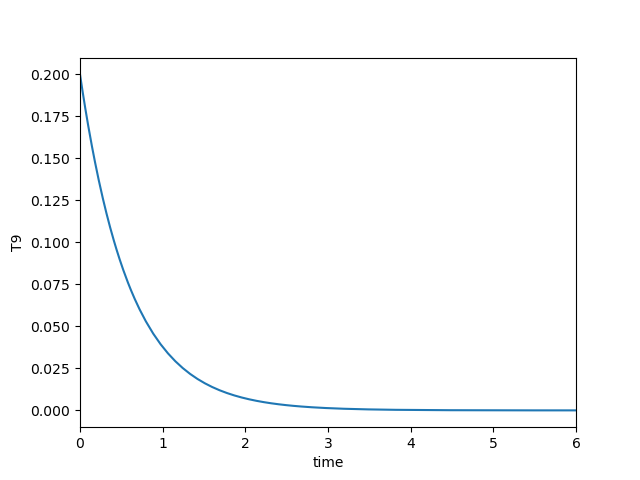
\includegraphics[width=0.75\textwidth]{Figures/Figure_1_exp.png}
    \caption{Temperature evolution for the exponential single-zone calculation. The temperature decreases rapidly from the initial value because of the imposed exponential expansion.}
    \label{fig:exp_t9}
\end{figure}

\subsection{Evolution of the CNO Diagnostic Ratio}

The abundance ratio (Equation~\ref{eq:ratio}) was calculated throughout the simulation. The initial value of this ratio is close to the solar-composition value. From the initial abundances, $X(^{14}\mathrm{N}) \simeq 7.97\times10^{-4}, X(^{15}\mathrm{N}) \simeq 3.14\times10^{-6}$, while the initial $^{14}\mathrm{O}$ and $^{15}\mathrm{O}$ abundances are very small. Therefore, the initial value of the ratio is approximately
\[
R_{15/14}^{\mathrm{initial}}
\approx
\frac{3.14\times10^{-6}}{7.97\times10^{-4}}
\approx 3.9\times10^{-3}.
\]

The calculation shows that $R_{15/14}$ first changes during the early active burning phase and then increases strongly before reaching a nearly constant freeze-out value. The final plateau is approximately
\[
R_{15/14}^{\mathrm{final}} \approx 0.4-0.5.
\]
This corresponds to an enhancement factor of roughly
\[
f_{\mathrm{enh}}
=
\frac{R_{15/14}^{\mathrm{final}}}
{R_{15/14}^{\mathrm{initial}}}
\sim 100.
\]

This result indicates that the exponential expansion model produces a significant enhancement of $^{15}\mathrm{N}$-rich material relative to the initial composition. The enhancement occurs because nuclear burning modifies the CNO isotopic distribution before the system cools and freezes out.

\begin{figure}[h!]
    \centering
    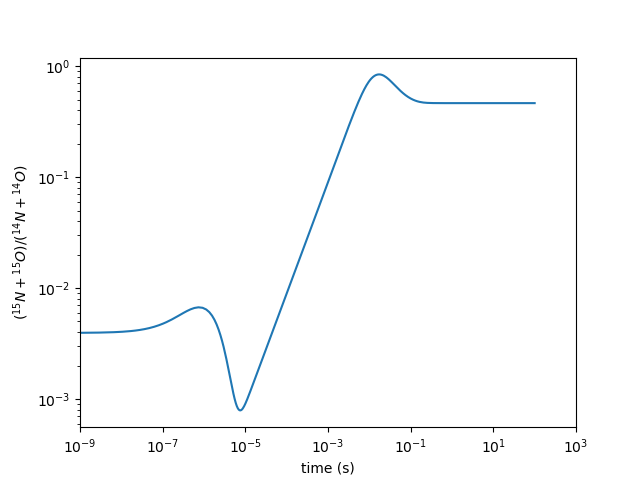
\includegraphics[width=0.75\textwidth]{Figures/Figure_2_exp.png}
    \caption{Evolution of the diagnostic abundance ratio $R_{15/14}$ for the exponential single-zone calculation. The ratio increases by about two orders of magnitude before reaching a freeze-out plateau.}
    \label{fig:exp_ratio}
\end{figure}

\section{Thermodynamic Trajectory Single-Zone Calculation}

\subsection{Trajectory Temperature and Density Evolution}

In the trajectory-based calculation, the temperature and density are not prescribed by a simple analytic function. Instead, they are read from a nova thermodynamic trajectory file. The calculation begins at a lower temperature than the exponential case and then follows a more complex nova-like evolution.

The trajectory begins near $T_9 \approx 0.091$, with a density of approximately $\rho \approx 2.21\times10^4~\mathrm{g~cm^{-3}}$. 
The temperature remains low during the early part of the calculation, then rises sharply and reaches a delayed maximum. After this peak, the temperature decreases again, and the nuclear reactions eventually freeze out.

This thermodynamic behaviour is very different from the exponential case. In the exponential calculation, the system begins hot and cools immediately. In the trajectory calculation, the system begins cooler, evolves for some time, and then experiences a strong heating phase. This delayed heating allows nuclear reactions to proceed under different conditions and produces a different final abundance pattern.

\begin{figure}[h!]
    \centering
    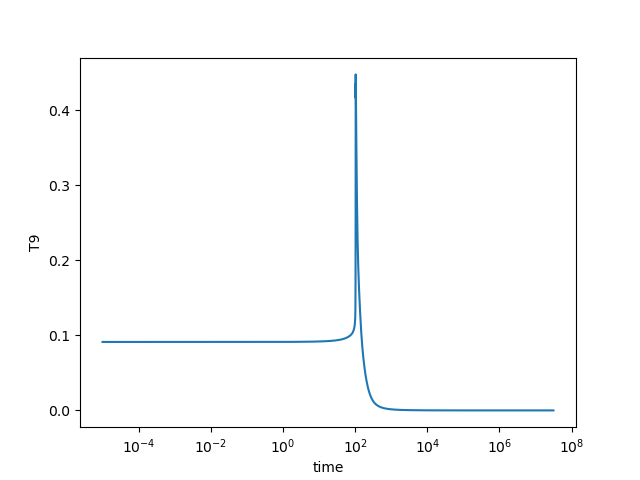
\includegraphics[width=0.75\textwidth]{Figures/Figure_1_traj.png}
    \caption{Temperature evolution for the trajectory-based single-zone calculation. The trajectory begins at relatively low temperature, later reaches a delayed temperature peak, and then cools toward freeze-out.}
    \label{fig:traj_t9}
\end{figure}

\subsection{Evolution of the CNO Diagnostic Ratio}

The same diagnostic ratio was calculated for the trajectory-based model. As in the exponential case, the initial value is close to
$ R_{15/14}^{\mathrm{initial}} \approx 4\times10^{-3}.$ During the early low-temperature phase, the ratio changes only slowly. As the trajectory approaches the temperature peak, proton-capture reactions become more efficient, and the hot-CNO reaction flow becomes stronger. This leads to a rapid modification of the $A=14$ and $A=15$ CNO abundances. After the temperature decreases, the reaction rates become too slow to maintain active burning, and the ratio reaches a final freeze-out plateau.

The final value of the ratio in the trajectory model is significantly larger than in the exponential model. The preliminary results show that $R_{15/14}^{\mathrm{final}}$ reaches a value of order a few. This means that the trajectory model produces a stronger enhancement of $^{15}\mathrm{N}$-rich material than the exponential model.

\begin{figure}[h!]
    \centering
    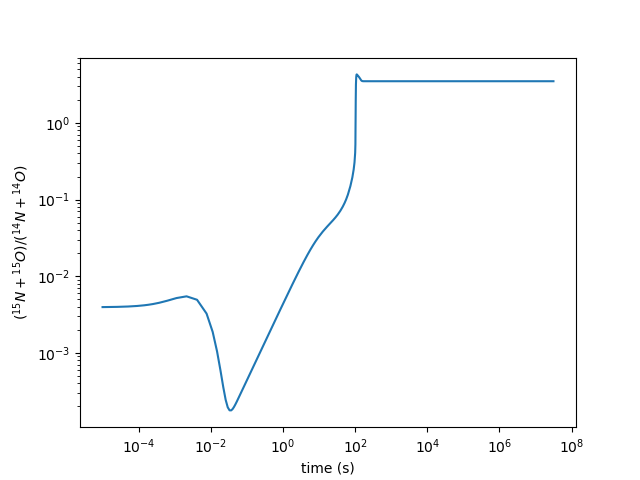
\includegraphics[width=0.75\textwidth]{Figures/Figure_2_traj.png}
    \caption{Evolution of the diagnostic abundance ratio $R_{15/14}$ for the trajectory-based single-zone calculation. The delayed temperature peak produces stronger hot-CNO processing and a larger final enhancement than in the exponential model.}
    \label{fig:traj_ratio}
\end{figure}

\section{Comparison Between the Exponential and Trajectory Calculations}

The two preliminary calculations demonstrate that the adopted thermodynamic history has a major effect on the final CNO isotopic composition. In the exponential case, the temperature starts at $T_9=0.20$ and decreases immediately. Therefore, most nuclear processing occurs at early times, and the abundance pattern freezes out rapidly. In contrast, the trajectory calculation begins at a lower temperature but later reaches a delayed temperature peak. This delayed heating phase allows stronger hot-CNO processing before freeze-out.

The most important difference is seen in the final value of the diagnostic ratio $R_{15/14}$. In the exponential model, the final value is approximately $R_{15/14}^{\mathrm{final}} \approx 0.4-0.5$, while in the trajectory model it reaches a value of order a few. Therefore, the trajectory model produces a stronger enhancement of $^{15}\mathrm{N}+^{15}\mathrm{O}$ relative to $^{14}\mathrm{N}+^{14}\mathrm{O}$.

\begin{table}[h!]
\centering
\caption{Summary of preliminary single-zone results.}
\begin{tabular}{llll}
\hline
Model & Thermodynamic behavior & Final $R_{15/14}$ & Interpretation \\
\hline
Exponential & Immediate cooling & $\sim 0.4-0.5$ & Early burning and freeze-out \\
Trajectory & Delayed temperature peak & order of a few & Stronger hot-CNO processing \\
\hline
\end{tabular}
\label{tab:preliminary_results}
\end{table}

These preliminary results suggest that the shape of the temperature-density history is not a minor detail. It directly affects the balance between proton captures, beta decays, and freeze-out. Therefore, realistic thermodynamic trajectories are essential for interpreting nova hydrogen burning and CNO isotope production.

\section{Physical Interpretation of the Preliminary Results}

The enhancement of $R_{15/14}$ can be understood as the result of competition between nuclear production and destruction channels in the hot-CNO cycle. Important reactions include $^{14}\mathrm{N}(p,\gamma)^{15}\mathrm{O}, ^{15}\mathrm{O}(\beta^+)^{15}\mathrm{N}, ^{15}\mathrm{N}(p,\alpha)^{12}\mathrm{C}$, and $ ^{15}\mathrm{N}(p,\gamma)^{16}\mathrm{O}$.

In the exponential model, the temperature decreases quickly. As a result, the time available for proton captures is limited. The system undergoes some active burning at early times, but the rapid cooling causes the abundances to freeze out before extended processing can occur.

In the trajectory model, the delayed temperature peak changes this behavior. The material remains in the burning environment until the temperature rises to a level where hot-CNO reactions become more efficient. This produces stronger processing of the CNO isotopes and a larger final value of $R_{15/14}$. Once the temperature decreases again, the nuclear reaction rates become slow and the abundance distribution freezes out.

Thus, the preliminary results indicate that the final CNO isotopic ratio depends not only on the maximum temperature, but also on the timing and duration of the heating and cooling phases.

\section{Future Work}

The preliminary calculations provide a strong starting point, but further analysis is required to fully understand the nucleosynthesis. The future work will focus on four main directions: larger nuclear networks, reaction-flow analysis, timescale analysis, and quasi-equilibrium behavior.

\subsection{Larger Nuclear Network Calculations}

The first step will be to extend the calculations to larger nuclear networks. The current preliminary results focus mainly on the CNO isotopic outcome. However, in nova environments, material can leak out of the CNO cycle into heavier reaction cycles, such as the Ne--Na and Mg--Al cycles. Therefore, it is necessary to determine whether the final value of $R_{15/14}$ is controlled only by local CNO cycling or whether it is affected by leakage into heavier nuclei.

Several network sizes will be considered as described in Table~\ref{tab:network_cases}. The final value of $R_{15/14}$ will be compared for each network. If the ratio remains nearly unchanged as the network size increases, this will indicate that the CNO result is robust and controlled mainly by local CNO reactions. If the ratio changes significantly, this will suggest that reactions involving heavier nuclei influence the final CNO isotopic composition.



\subsection{Reaction-Flow Analysis}

The second step will be to calculate the dominant reaction flows during the burning phase. Reaction-flow analysis will show which nuclear pathways are responsible for the production and destruction of the key CNO isotopes. For proton-capture reactions, the flow is represented by Equation~\ref{eq:flow} and for beta decays as in Equation~\ref{eq:betaflows}. The main reactions to be examined include $^{12}\mathrm{C}(p,\gamma)^{13}\mathrm{N}, ^{13}\mathrm{N}(p,\gamma)^{14}\mathrm{O}, ^{14}\mathrm{N}(p,\gamma)^{15}\mathrm{O}, ^{14}\mathrm{O}(\beta^+)^{14}\mathrm{N}, ^{15}\mathrm{O}(\beta^+)^{15}\mathrm{N}, \\ ^{15}\mathrm{N}  (p,\alpha)^{12}\mathrm{C}, $ and $^{15}\mathrm{N}(p,\gamma)^{16}\mathrm{O}. $
This analysis will help identify the dominant pathways and nuclear bottlenecks in both the exponential and trajectory-based calculations.

\subsection{Timescale Analysis}

The third step will be to compute nuclear and thermodynamic timescales. This analysis will determine when nuclear reactions can keep up with the changing thermodynamic conditions and when freeze-out occurs.

If the nuclear timescale is shorter than the thermodynamic timescale, the reaction can proceed efficiently. If the nuclear timescale becomes longer than the thermodynamic timescale, the reaction freezes out. Comparing these timescales will provide a physical explanation for the different final abundance ratios found in the exponential and trajectory models.

\subsection{Quasi-Equilibrium and Freeze-Out}

The final step will be to investigate whether the CNO cycle approaches quasi-equilibrium or steady-flow behaviour during the active burning phase. At nova temperatures, full nuclear statistical equilibrium is not expected. However, parts of the CNO cycle may temporarily approach a quasi-steady flow. This can be tested by comparing reaction flows around the CNO cycle. A simple steady-flow condition may be written as
\[
F_{^{12}\mathrm{C}(p,\gamma)}
\approx
F_{^{13}\mathrm{N}(p,\gamma)}
\approx
F_{^{14}\mathrm{N}(p,\gamma)}
\approx
F_{^{15}\mathrm{N}(p,\alpha)} .
\]

If these flows are approximately equal, the CNO cycle is close to steady flow. If one flow is much smaller than the others, that reaction acts as a bottleneck. The breakdown of this balance will be interpreted as the onset of freeze-out or departure from quasi-equilibrium.

\section{Summary}

The preliminary single-zone calculations show that nova hydrogen burning is strongly influenced by the adopted thermodynamic history. The exponential model produces rapid early burning followed by freeze-out and enhances $R_{15/14}$ by about two orders of magnitude. The trajectory-based model produces a stronger final enhancement because its delayed temperature peak allows more efficient hot-CNO processing.

The future work will extend these preliminary results by performing larger network calculations, analysing reaction flows, computing nuclear and thermodynamic timescales, and studying quasi-equilibrium behaviour. These steps will provide a more complete physical interpretation of CNO isotope production and freeze-out in nova hydrogen burning. % Experimental Setup
%\addtotoc{chapter4}
%% Chapter 4

\chapter{Conclusion} % Write in your own chapter title
\label{Chapter4}
\lhead{Chapter 3. \emph{Conclusion}} % Write in your own chapter title to set the page header
\fancyfoot[CE,CO]{\hline \\ \small M.Sc. Thesis • Student's name  • Dep. of Applied Physics and Astronomy • UoS • 2025}
At the end we Studied \ldots. % Experiment 1

%\input{./Chapters/Chapter5} % Experiment 2

%\input{./Chapters/Chapter6} % Results and Discussion

%\input{./Chapters/Chapter7} % Conclusion

%% ----------------------------------------------------------------
% Now begin the Appendices, including them as separate files

%\addtocontents{toc}{\vspace{2em}} % Add a gap in the Contents, for aesthetics

%\appendix % Cue to tell LaTeX that the following 'chapters' are Appendices

%\input{./Appendices/AppendixA}	% Appendix Title

%\input{./Appendices/AppendixB} % Appendix Title

%\input{./Appendices/AppendixC} % Appendix Title

%\addtocontents{toc}{\vspace{2em}}  % Add a gap in the Contents, for aesthetics

%\backmatter

%% ----------------------------------------------------------------

\label{Bibliography}
%\lhead{\emph{Bibliography}}  % Change the left side page header to "Bibliography"
%\bibliographystyle{unsrtnat}  % Use the "unsrtnat" BibTeX style for formatting the Bibliography
%\bibliographystyle{nature}
%\bibliographystyle{abbrv}
%\bibliographystyle{stylename}
%\bibliographystyle{authoryear}
%\bibliographystyle{aasjournal}
\bibliography{Bibliography}  % The references (bibliography) information are stored in the file named "Bibliography.bib"

\end{document}  % The End
%% ----------------------------------------------------------------